% Figure for the proof of prop:superpoly (nested shells), \input at the end of the
% paragraph "Wire the shells in increasing order of radius ...".
\begin{figure}[ht]
\centering
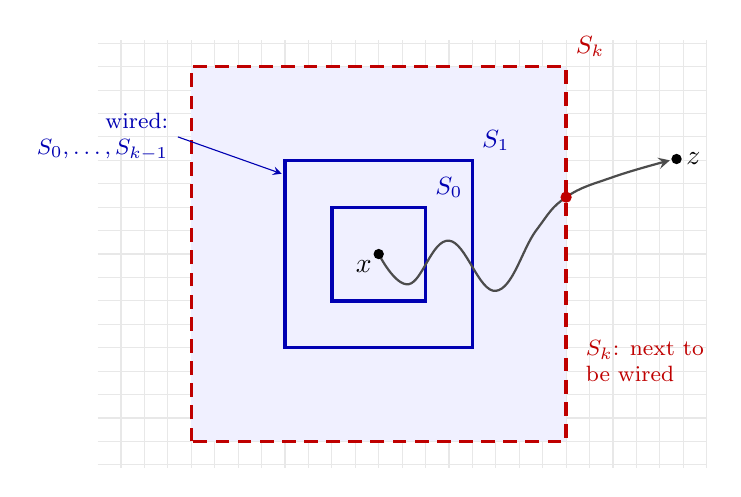
\begin{tikzpicture}[scale=0.85,
    wired/.style={very thick, blue!70!black},
    next/.style={very thick, red!75!black, dash pattern=on 5pt off 3pt},
    later/.style={thick, gray!60}]
  % lattice background
  \draw[step=0.35, gray!18] (-4.2,-3.2) grid (4.9,3.2);
  % region where all previous identifications live
  \fill[blue!6] (-2.8,-2.8) rectangle (2.8,2.8);
  % wired shells S_0, S_1 (here k = 2)
  \draw[wired] (-0.7,-0.7) rectangle (0.7,0.7);
  \draw[wired] (-1.4,-1.4) rectangle (1.4,1.4);
  % the next shell S_k
  \draw[next] (-2.8,-2.8) rectangle (2.8,2.8);
  % a path from x to z
  \draw[thick, black!70, ->, >=stealth]
    plot[smooth, tension=0.7] coordinates
      {(0,0) (0.45,-0.45) (1.05,0.2) (1.75,-0.55) (2.35,0.35) (2.8,0.85) (3.5,1.15) (4.35,1.4)};
  \fill[red!75!black] (2.8,0.85) circle (2.4pt);
  % points
  \fill (0,0) circle (2.2pt) node[below left=-1pt] {$x$};
  \fill (4.45,1.42) circle (2.2pt) node[right] {$z$};
  % labels
  \node[blue!70!black, anchor=south west, font=\small] at (0.7,0.7) {$S_0$};
  \node[blue!70!black, anchor=south west, font=\small] at (1.4,1.4) {$S_1$};
  \node[red!75!black, anchor=south west, font=\small] at (2.8,2.8) {$S_k$};
  \node[blue!70!black, align=right, font=\footnotesize, anchor=east] (w) at (-3.0,1.75)
    {wired:\\ $S_0,\dots,S_{k-1}$};
  \draw[->, >=stealth, blue!70!black] (w.east) -- (-1.45,1.2);
  \node[red!75!black, align=left, font=\footnotesize, anchor=west] at (2.95,-1.6)
    {$S_k$: next to\\ be wired};
\end{tikzpicture}
\caption{Wiring the nested shells in increasing order of radius (shown for $k=2$).
The boundaries $S_0,\dots,S_{k-1}$ (solid) are already wired, each to a single vertex;
all these identifications take place in the shaded region strictly inside $S_k$
(dashed). Every path from $x$ to $z$ still meets $S_k$ (dot), so $S_k$ separates $x$
from $z$ in the wired graph and \cref{prop:separator-wiring} applies again.}
\label{fig:nested-shells}
\end{figure}
